
%*****************************************
\chapter{Theoretical Foundation and Hypotheses}\label{ch:third}
%*****************************************

In the following chapter, we will present an unpublished scientific work that will serve as the theoretical core of our thesis. This scientific paper goes by the title 
\begin{center}
 \textit{"Designing Efficient Authentication Mechanisms: There is More to Efficiency than Input Speed."}   
\end{center}
Thus the authors remain unknown. We will refer to them as Anonymous et al. \cite{anonymous} in the following course of this thesis. As implied in Section \ref{2.2}, our intention for this chapter is to introduce an interesting contribution made towards setting a standard for the evaluation of efficiency in smartphone authentication mechanisms. We will begin by presenting the findings of Anonymous et al. \cite{anonymous}. Then, we will proceed by elaborating on the limitations of their approach. Lastly, we will explain how we intend to validate their findings by reevaluating their approach and proving their hypotheses.

\section{Approach}

As discussed in Chapter \ref{ch:second}, the lack of usability in various authentication mechanisms, has been the main reason why many smartphone users refuse to use a screen lock for their phones. In Section \ref{2.2}, we saw how researchers attempted to make authentication mechanisms more usable by increasing their perceived effectiveness. Unfortunately, this approach was only successful to a certain extent and was not sufficiently productive for solving the usability issue. We learned that users generally value efficiency over effectiveness when it comes to authentication mechanisms and would prefer no screen lock rather than using one that is time-consuming and inconvenient (see Section \ref{2.2}). Consequently, researchers tried to detect the factors that most affected the efficiency of smartphone security and realized that these factors could not be assessed by simply measuring the duration of the input. They noticed a factor that had often been disregarded during the evaluation of efficiency, and that is \textit{mental effort} (see Section \ref{2.2}). The amount of mental effort that is needed to accomplish an authentication task is crucial for user-acceptance \cite{anonymous}. Therefore, new measurement methods are in need which approach the practice of authentication on a human level and are designed with respect to humans' perception of time and cognitive abilities. \\


To that, Anonymous et al. \cite{anonymous} made an effort to create a measurement standard for evaluating the usability of authentication mechanisms in terms of their efficiency \cite{anonymous}. They noticed how previous studies indicated that users commonly prefer authentication mechanisms that require little to no mental effort \cite{anonymous, AnatomySmartphone}. Moreover, they realized that those mechanisms were the ones to be rated most usable and fastest to use. Researchers made these revelations possible, by categorizing the overall authentication time into \textbf{orientation} and \textbf{input} times \cite{anonymous}. Anonymous et al. \cite{anonymous} also analyzed the danger that occurred from only considering input times in evaluations. Thus it can lead to false conclusions about the efficiency of authentication mechanisms. This is specially the case when mechanisms are set in comparison to each other \cite{anonymous}. \\

\begin{figure}[t!]
\centering
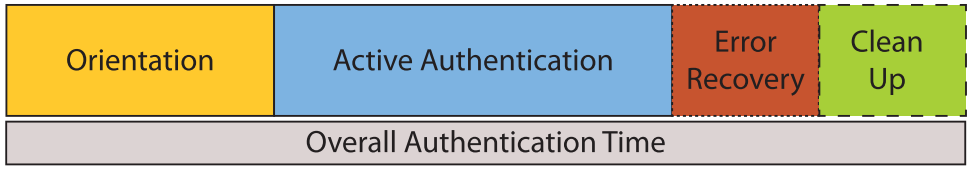
\includegraphics[width=13cm, height=2cm]{Chapters/graphics/Phases.PNG}
\caption{Component phases of an authentication process. While Orientation and Active Authentication (input) phase are the core components of an authentication procedure, Error Recovery may also be included. Clean up phases are not considered part of the authentication process, yet in some designs they are crucial for its completeness \cite{anonymous}. }
\label{fig:phases}
\end{figure}

Anonymous et al. \cite{anonymous} began by reinterpreting the architecture of the general smartphone authentication process (see figure \ref{fig:phases}). Next, they subdivided the overall authentication period into the following phases \cite{anonymous}: 

\begin{itemize}
    \item \textbf{\textcolor{orange}{Orientation:}} In previous research, this phase was commonly defined as the \textit{preparation} phase \cite{anonymous}. It defines the period, beginning from the moment a smartphone screen is switched on, to the moment when the first input action is made \cite{anonymous}. It usually takes place before the user enters their secret. This is the time which they spend either recalling their secret, preparing themselves for its input, or both \cite{anonymous}. It is considered to be the part of the authentication process which requires the most mental effort \cite{anonymous}.  
    \item \textbf{\textcolor{blue}{Active Authentication:}} This phase defines the time a user needs to enter their secret. It begins with the very first input action and ends with the very last\footnote{By \textit{last input action}, we mean the moment which determines whether unlocking is permitted or denied \cite{anonymous}.}. We will call this phase the \textbf{input} phase, for simplicity reasons.
    \item \textbf{\textcolor{red}{Error Recovery:}} This phase is useful in situations where the user makes an input error. Its purpose is to signify the user that an error has occurred and to provide the possibility of recovering from it by making the user restart the authentication process, or by allowing so called \textit{undo operations}, which allow the user to correct their mistake and proceed with the input. 
    \item \textbf{\textcolor{green}{Clean Up:}} This phase is not considered to be a solid part of the authentication process, yet in some newly developed mechanisms, it is crucial for completing the authentication. An example for its use, is found in the concepts \textbf{TinyLock} by Kwon et al. \cite{kwon} and \textbf{Whispercore} by Airowaily et al. \cite{Airowaily}. In these designs, the clean up phase is intended to remove oily residues on the smartphone screen and thereby counteract the chance of potential smudge attacks \cite{anonymous}. 
\end{itemize}

The two phases which are considered to be highly essential for the authentication process are the \textit{orientation} and \textit{input} phases. In previous approaches, the \textit{input} phase has often been considered to define the actual authentication procedure. Consequently, \textit{orientation} time was often disregarded and ignored in usability evaluations. \textit{Error recovery} is a phase that is not essentially mandatory for authentication, yet very useful for error management. Anonymous et al. \cite{anonymous} find that its implementation can have a significant effect on the efficiency of an authentication mechanism. In some cases, its implementation can cause for further \textit{orientation} or \textit{clean up} phases \cite{anonymous}. This, in return, may cause a longer authentication duration. The implementation of the \textit{clean up} phase depends on the design of the authentication concept. Authentication is possible with or without it. \\

By outlining the structure of the authentication process, Anonymous et al. \cite{anonymous} made a collection of observations and factors which they wanted to regard and prove in a user case study. First, they wanted to consider how authentication phases are proportioned. Reason being that it has a significant influence on the perceived efficiency of mechanisms. Moreover, the longer the \textit{orientation} time of an authentication mechanism is, the slower and less efficient it is perceived. In fact, cases in which the duration of the \textit{orientation} phase exceeds the \textit{input} phase, have been seen to be widely disliked by users. \\

Second, they wanted to consider how authentication phases are ordered in an authentication process \cite{anonymous}. Thus this factor may highly differ amongst authentication concepts, such as Pattern Rotation and Marbles \cite{Marbles} (Section \ref{2.2.3}), it is very important to regard. For instance, Pattern Rotation only consists of two phases, with the \textit{orientation} phase preceding the \textit{input} phase. Marbles, on the other hand, has multiple small \textit{orientation} and \textit{input} phases, ordered in an alternating manner. Interestingly, Anonymous et al. \cite{anonymous} find that the latter has the possibility of decreasing the perceived duration of authentication. \\

Third, they want to regard the coherence of \textit{orientation} and \textit{input} phases in terms of their contexts. Thus it also has a significant impact on a mechanism's perceived efficiency \cite{anonymous}. Meaning, the less coherent the contexts of \textit{orientation} time and \textit{input} time are, the less efficient and convenient they are perceived. This factor was regarded in the design of Marbles \cite{Marbles}. Thus its tasks alternate between finding the marbles and entering them, the contexts of the tasks complement each other. Through further research Anonymous et al. \cite{anonymous} found that humans tend to perceive periods longer than they are if the contexts of these periods are incoherent \cite{anonymous,perception}.\\

Lastly, Anonymous et al. \cite{anonymous} state that \textit{error recovery} should be cautiously managed throughout the authentication of a mechanism \cite{anonymous}. As mentioned above, the implementation of \textit{error recovery} may result in further \textit{orientation} and \textit{clean up} phases. This observation was shown in findings by Zezschwitz et al. \cite{PatternWild}, discussed in section \ref{2.2}. They discovered how users tended more towards Pattern authentication than Pin because it managed errors better. Even though Pattern took longer to authenticate with than Pin. This is because Pin allowed to manage errors through \textit{undo-operations}. These have shown to be disliked and therefore are seldom used in designs \cite{PatternWild, anonymous}. 

\begin{figure}[t!]
\centering
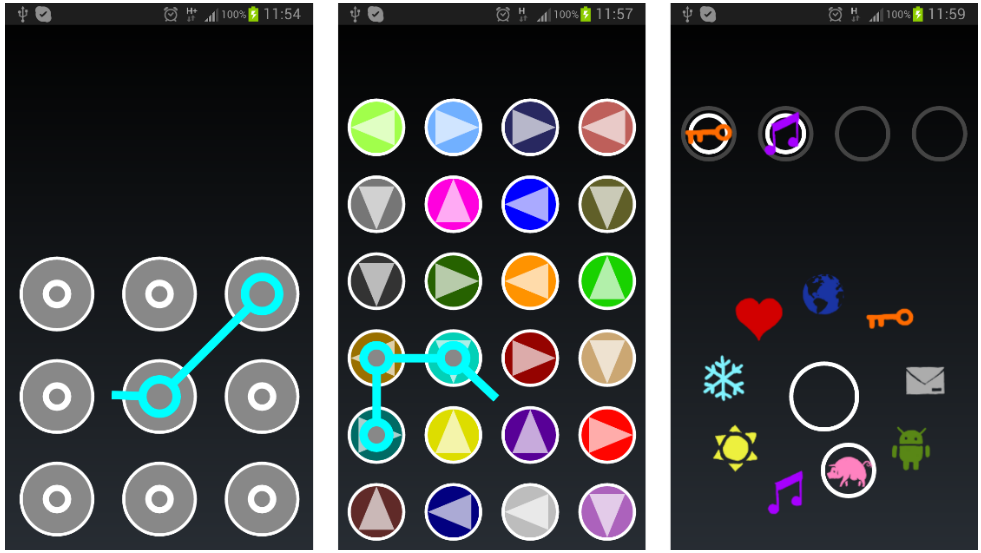
\includegraphics[width=14cm, height=7cm]{Chapters/graphics/androidPatternMarble.PNG}
\caption{The concepts that Anonymous et al. \cite{anonymous} used in their study. Left: Android Unlock Pattern (baseline); Middle: Pattern Rotation; Right: Marbles. See figure \ref{fig:marbles} to see how the concepts were modified \cite{anonymous}.}
\label{fig:android}
\end{figure}

\section{User Case Study}

To prove their assumptions and observations, Anonymous et al. \cite{anonymous} decided to focus mainly on the phases, \textit{orientation}, and \textit{input}. Thus they are the most important phases during authentication. They selected three authentication concepts, each representing a different ratio of \textit{orientation} and \textit{input} time \cite{anonymous}
\footnote{To better understand the functionalities of the concepts listed above, we recommend revisiting the approach by Zezschwitz et al. \cite{Marbles}, presented in Section \ref{2.2.3}.}: 

\begin{itemize}
    \item \textbf{Android Unlock Pattern} presented a \textcolor{red}{short} orientation - \textcolor{red}{short} input ratio,
    \item \textbf{Pattern Rotation} presented a \textcolor{blue}{long} orientation - \textcolor{red}{short} input ratio,
    \item \textbf{Marbles} presented a ratio in which orientation and input time were interlaced.
\end{itemize}

It is important to note that \textit{Pattern Rotation} and \textit{Marbles} \cite{Marbles} were slightly modified in this study. \textit{Pattern Rotation} presented a larger grid than the original design, and in \textit{Marbles}, the elements (marbles) were small images rather than colors only (see figure \ref{fig:android} and \ref{fig:marbles}. All three concepts were implemented in a prototype which was intended to be installed on the Android smartphones of study participants \cite{anonymous}. The prototype was intended to serve as an authentication system on the participants' phones. Each of the concepts was planned to be tested for ten days \cite{anonymous}. After each ten-day period, an online survey was required to be taken. Also, during the concept-tests, \textit{orientation} and \textit{input} times were logged for each authentication \cite{anonymous}. \textit{Orientation} time was logged from the moment the screen was switched on, to the first input event. \textit{Input} time was logged from the first to the last input event \cite{anonymous}. Participants were allowed to choose their secrets for the concepts. However, patterns for \textit{Android Unlock Pattern} had to consist of six nodes, patterns for \textit{Pattern Rotation} had to have five nodes, and secrets in \textit{Marbles} had to consist of four elements \cite{anonymous}.

\subsection{Results}

The study yielded 19 participants and delivered a set of 18 valid data entities \cite{anonymous}. Anonymous et al. \cite{anonymous} wanted to examine the different outcomes that result when authentication times are analyzed differently. First, they analyzed the overall authentication times of the concepts and noted the following ranking in regarding the \textbf{measured performances}\footnote{The concepts are ordered from fastest to slowest (or best to worst) in this and the following rankings of this section.} \cite{anonymous}:

\begin{enumerate}
    \item \textbf{Android Unlock Pattern},
    \item \textbf{Pattern Rotation},
    \item \textbf{Marbles}.
\end{enumerate} 

However, when they analyzed the \textit{input} times of each other concepts only, they noticed the following difference:

\begin{enumerate}
    \item \textbf{Pattern Rotation},
    \item \textbf{Android Unlock Pattern},
    \item \textbf{Marbles}.
\end{enumerate}

Last, they analyzed the \textit{orientation} time of the concepts and realized another significantly different outcome. \textit{Android Pattern Unlock} required the least amount of mental effort and therefore had the shortest \textit{orientation} time, on average \cite{anonymous}. Interestingly, there was hardly any difference between \textit{Pattern Rotation} and \textit{Marbles}, in terms of their average \textit{orientation} times \cite{anonymous}. The \textbf{perceived efficiency} of the concepts was rated qualitatively through five-point Likert scales \cite{anonymous}. Results showed that \textit{Android Unlock Pattern} was seen as the fastest of all three concepts. More than half of the participants considered \textit{Marbles} to be efficient, despite it being measured slower than \textit{Pattern Rotation}. Moreover, half of the participants perceived \textit{Pattern Rotation} as efficient \cite{anonymous}. Also, participants ranked the concepts in the following when asked if they contented a fast and easy orientation \cite{anonymous}: 

\begin{enumerate}
     \item \textbf{Android Unlock Pattern},
    \item \textbf{Marbles},
    \item \textbf{Pattern Rotation}.
\end{enumerate}

Lastly, when asked about the required cognitive effort, all participants approved of Android Pattern Unlock requiring the least amount of mental effort, followed by Pattern Rotation, then Marbles \cite{anonymous}. \\

\textcolor{red}{STILL HAVE TO ANALYZE THE RESULTS}

\section{Limitations and suggestive improvements}

In this section, we will first begin by reporting some limitations of the study, given by Anonymous et al. \cite{anonymous}. Then we will proceed by sharing our observations on specific qualities of the study, which we attempt to modify and improve to make their findings and observations universally valid.  

First, Anonymous et al. \cite{anonymous} state that the overall perception of the tested concepts could have been influenced by the participants' general preference \cite{anonymous} because a person's culture and history have shown to influence their acceptance of a particular system \cite{Harbach:2016} (Section \ref{2.2.1}). We intend to exclude this limitation by developing a prototype in which the particular ratios are represented through the same concept. That way, we will, hopefully, receive more a genuine evaluation of the ratios, without any interference of participants' preferences regarding a particular concept. Moreover, Anonymous et al. \cite{anonymous} state that the measured times for \textit{orientation} might differ from the actual times \cite{anonymous}. Reason being that the measurements for the \textit{orientation} times began as soon as the smartphone screen was turned on, and it is not guaranteed that authentication was the only immediate action after this event \cite{anonymous}. We plan on rectifying this possible inaccuracy, by isolating the \textit{orientation} phase from any other possible action. We will design our concept in a way that requires the user to initiate the authentication process actively, such that we can define a fix starting point for the \textit{orientation} time for the measurement.\\

Furthermore, the chosen ratios by Anonymous et al. \cite{anonymous} might not have been suitable enough to receive a definite result on whether users truly prefer short \textit{orientation} over long \textit{orientation}. We think it would be interesting to observe the outcome of testing ratios that have the same temporal arrangement, yet are contrasting regarding the lengths of their phases. Thus not included by Anonymous et al., we consider including the ratio \textit{short orientation - long input} into our analysis. We imagine that by mainly focusing on the ratios \textit{long orientation - short input} and \textit{short orientation - long input}, and by setting the ratio \textit{short orientation - short input} ratio as a baseline, we could receive more detailed results on users' attitude towards authentication concepts with different lengths of \textit{orientation} phases. Also, we could observe how far different lengths of \textit{input} phases might play a role in their preference and perception of efficiency. Lastly, we suggest that by letting participants qualitatively evaluate the ratios in comparison to each other, we hope to receive more detailed and precise information about their preferences.  







